\section{Method}
\label{Method}
%
The study where conducted on Danish travellers who interacted with a social robot in a natural setting, which in this study is Aalborg Airport (AAL). The study was conducted after the travellers went through the security check and before they reached the shopping and dining area at the airport. The travellers who interact with the robot are asked to participate in a semi-structured interview about their first impressions while being observed during both the interaction and the interview. 

\subsection{Materials}
For the study a \textit{Double 1} robot from Double Robotics Inc. with an iPad Air 2 is used. In relation to the current study it is decided to change the head mount so the iPad is angled upwards. The modified \textit{Double 1} robot is shown on \autoref{fig:ModificeretDoubleFront} and \autoref{fig:ModificeretDoubleSideClose}. The \textit{Double 1} robot was connected to a laptop via WiFi connection and its own software. \textit{Double 1} software allows a web page to be superimposed on the iPad screen while the observer still is able to control the robot from the laptop. It is not possible to control \textit{Double 1} when an application other than the \textit{Double 1} software is running. A wireframe was developed in \textit{Marvel} (\url{www.marvelapp.com}) to depict the potential usage of the robot in AAL, which will be the web page presented on the iPad. The wireframe is meant to simulate a wayfinding tool specific to the airport. The entire wireframe is formulated in Danish due to the fact that the study only involves Danish travellers.
%
\begin{figure}[H]
\centering
\begin{minipage}{.25\textwidth}
  \centering
  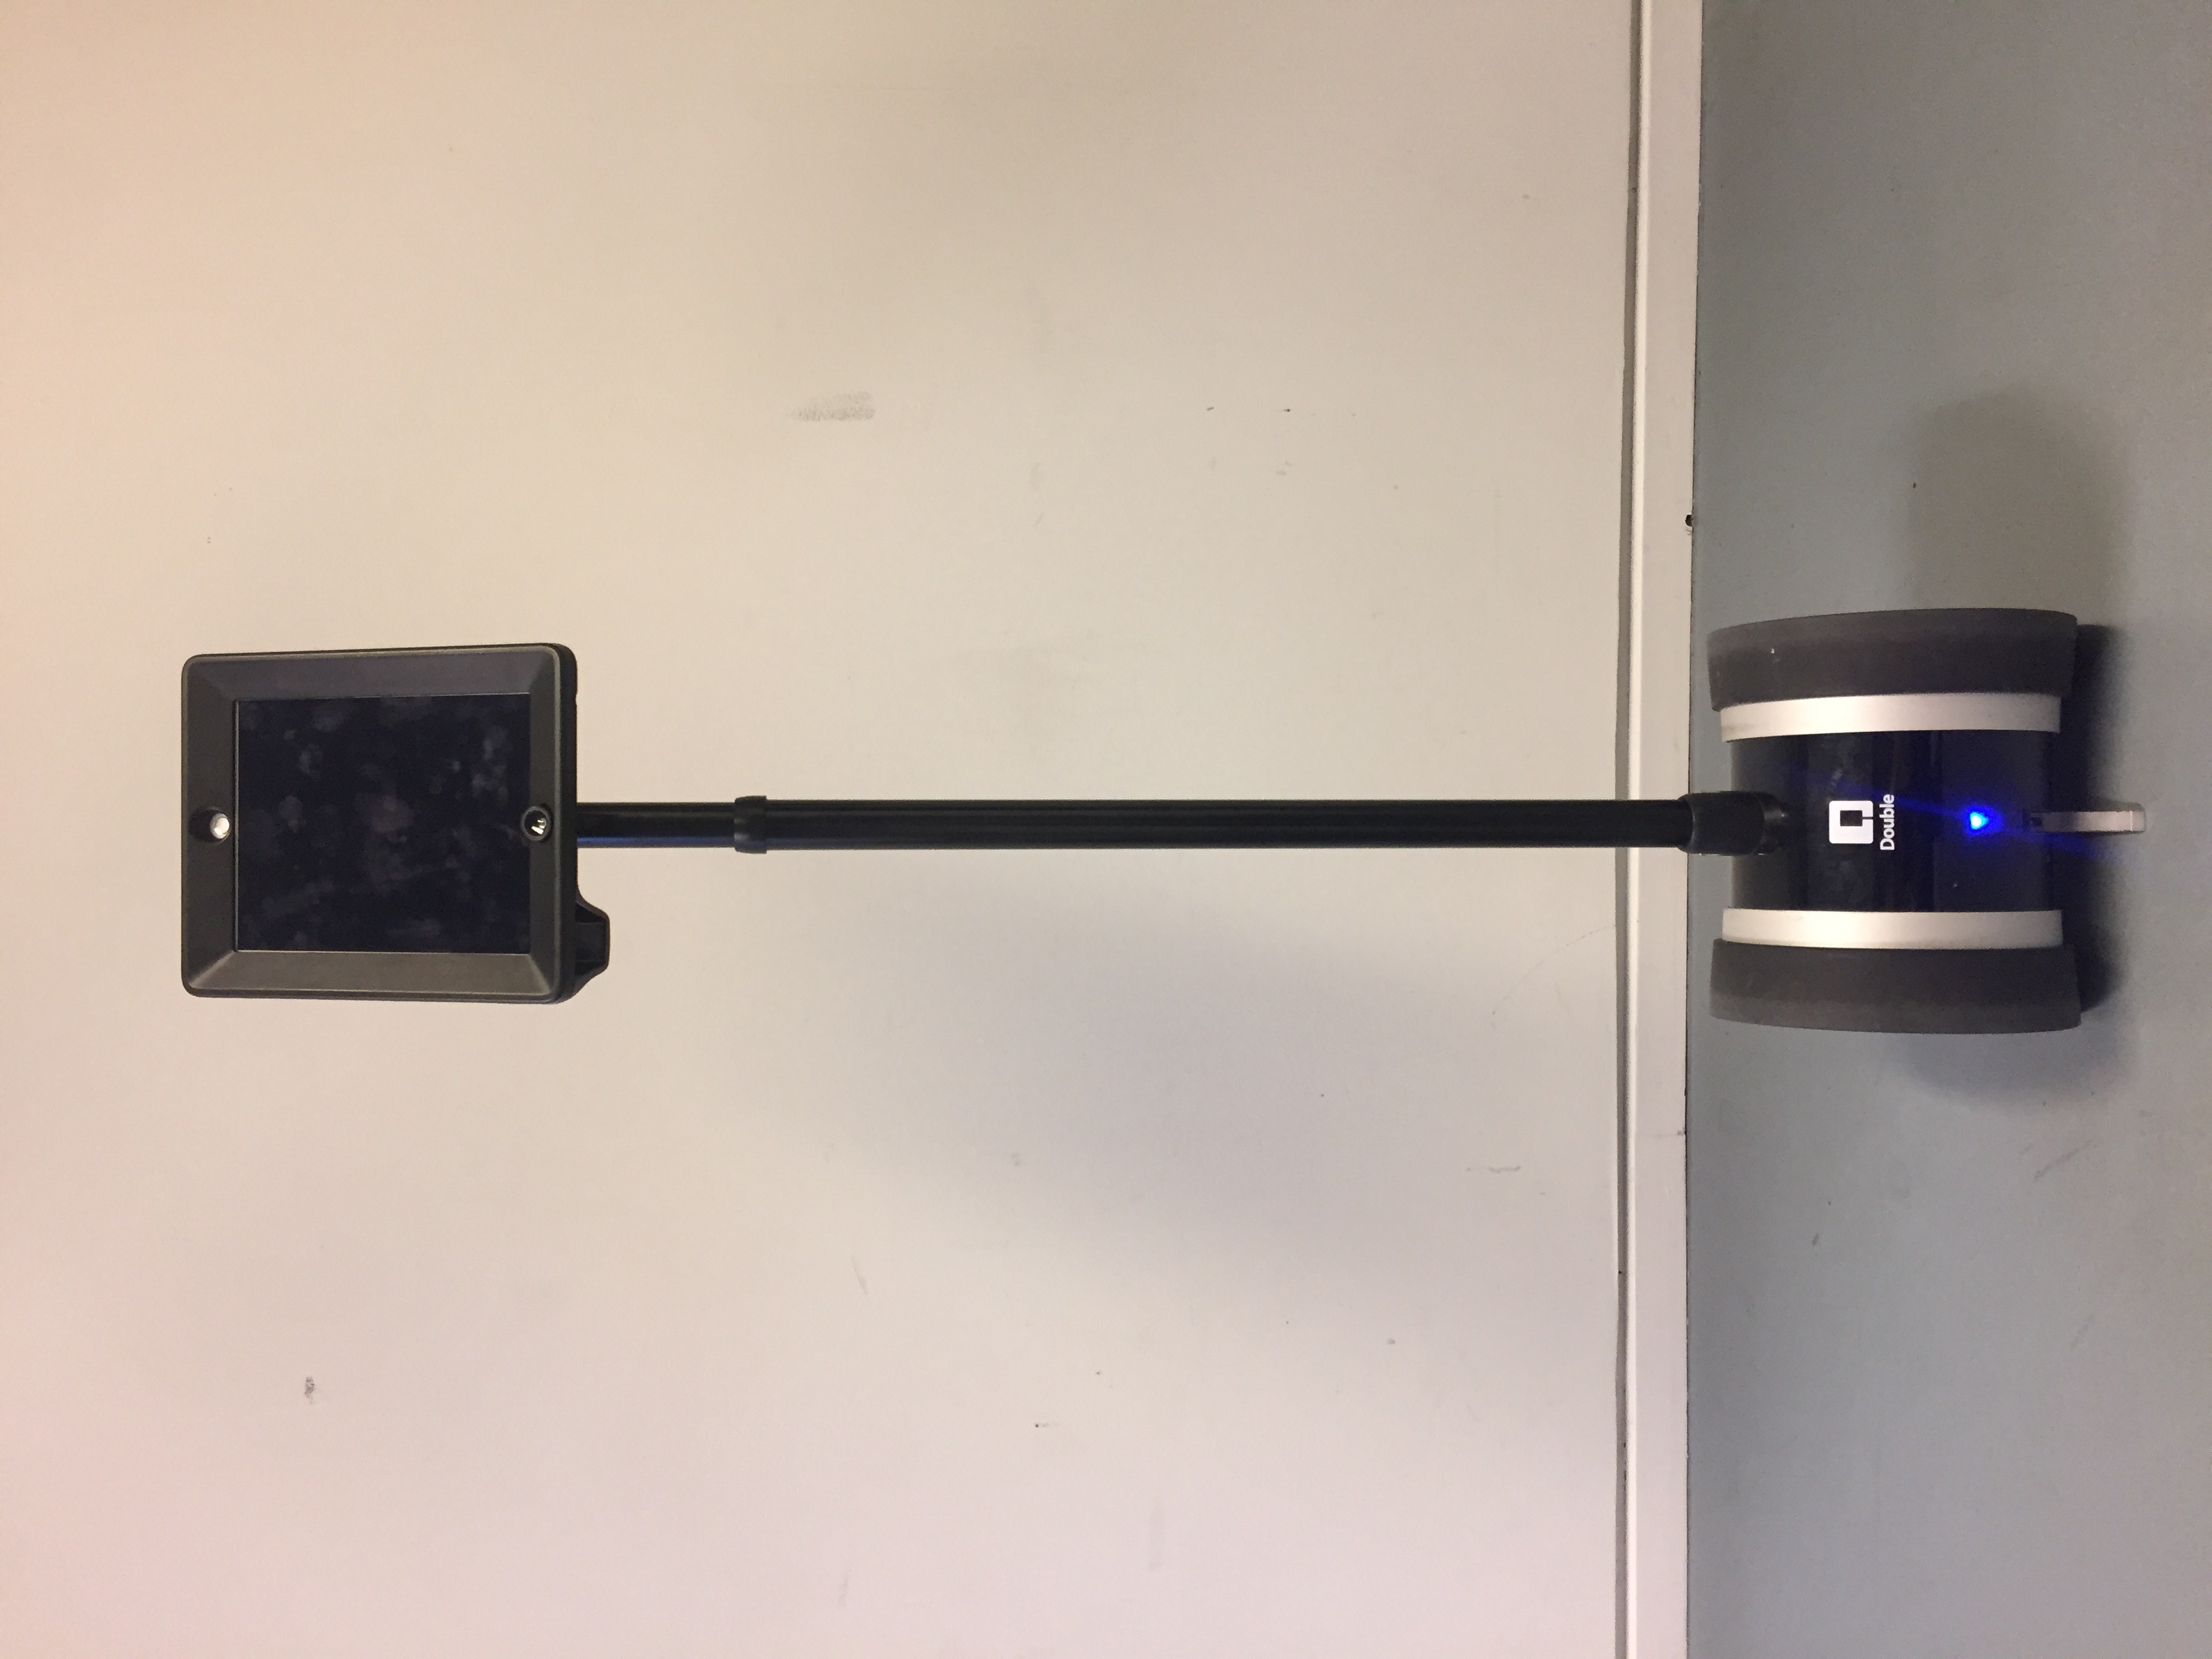
\includegraphics[width=\linewidth, angle =-90]{Figure/ModificeretDoubleFront}
  \caption{\textit{Double} front.}
  \label{fig:ModificeretDoubleFront}
\end{minipage}%
\begin{minipage}{.25\textwidth}
  \centering
  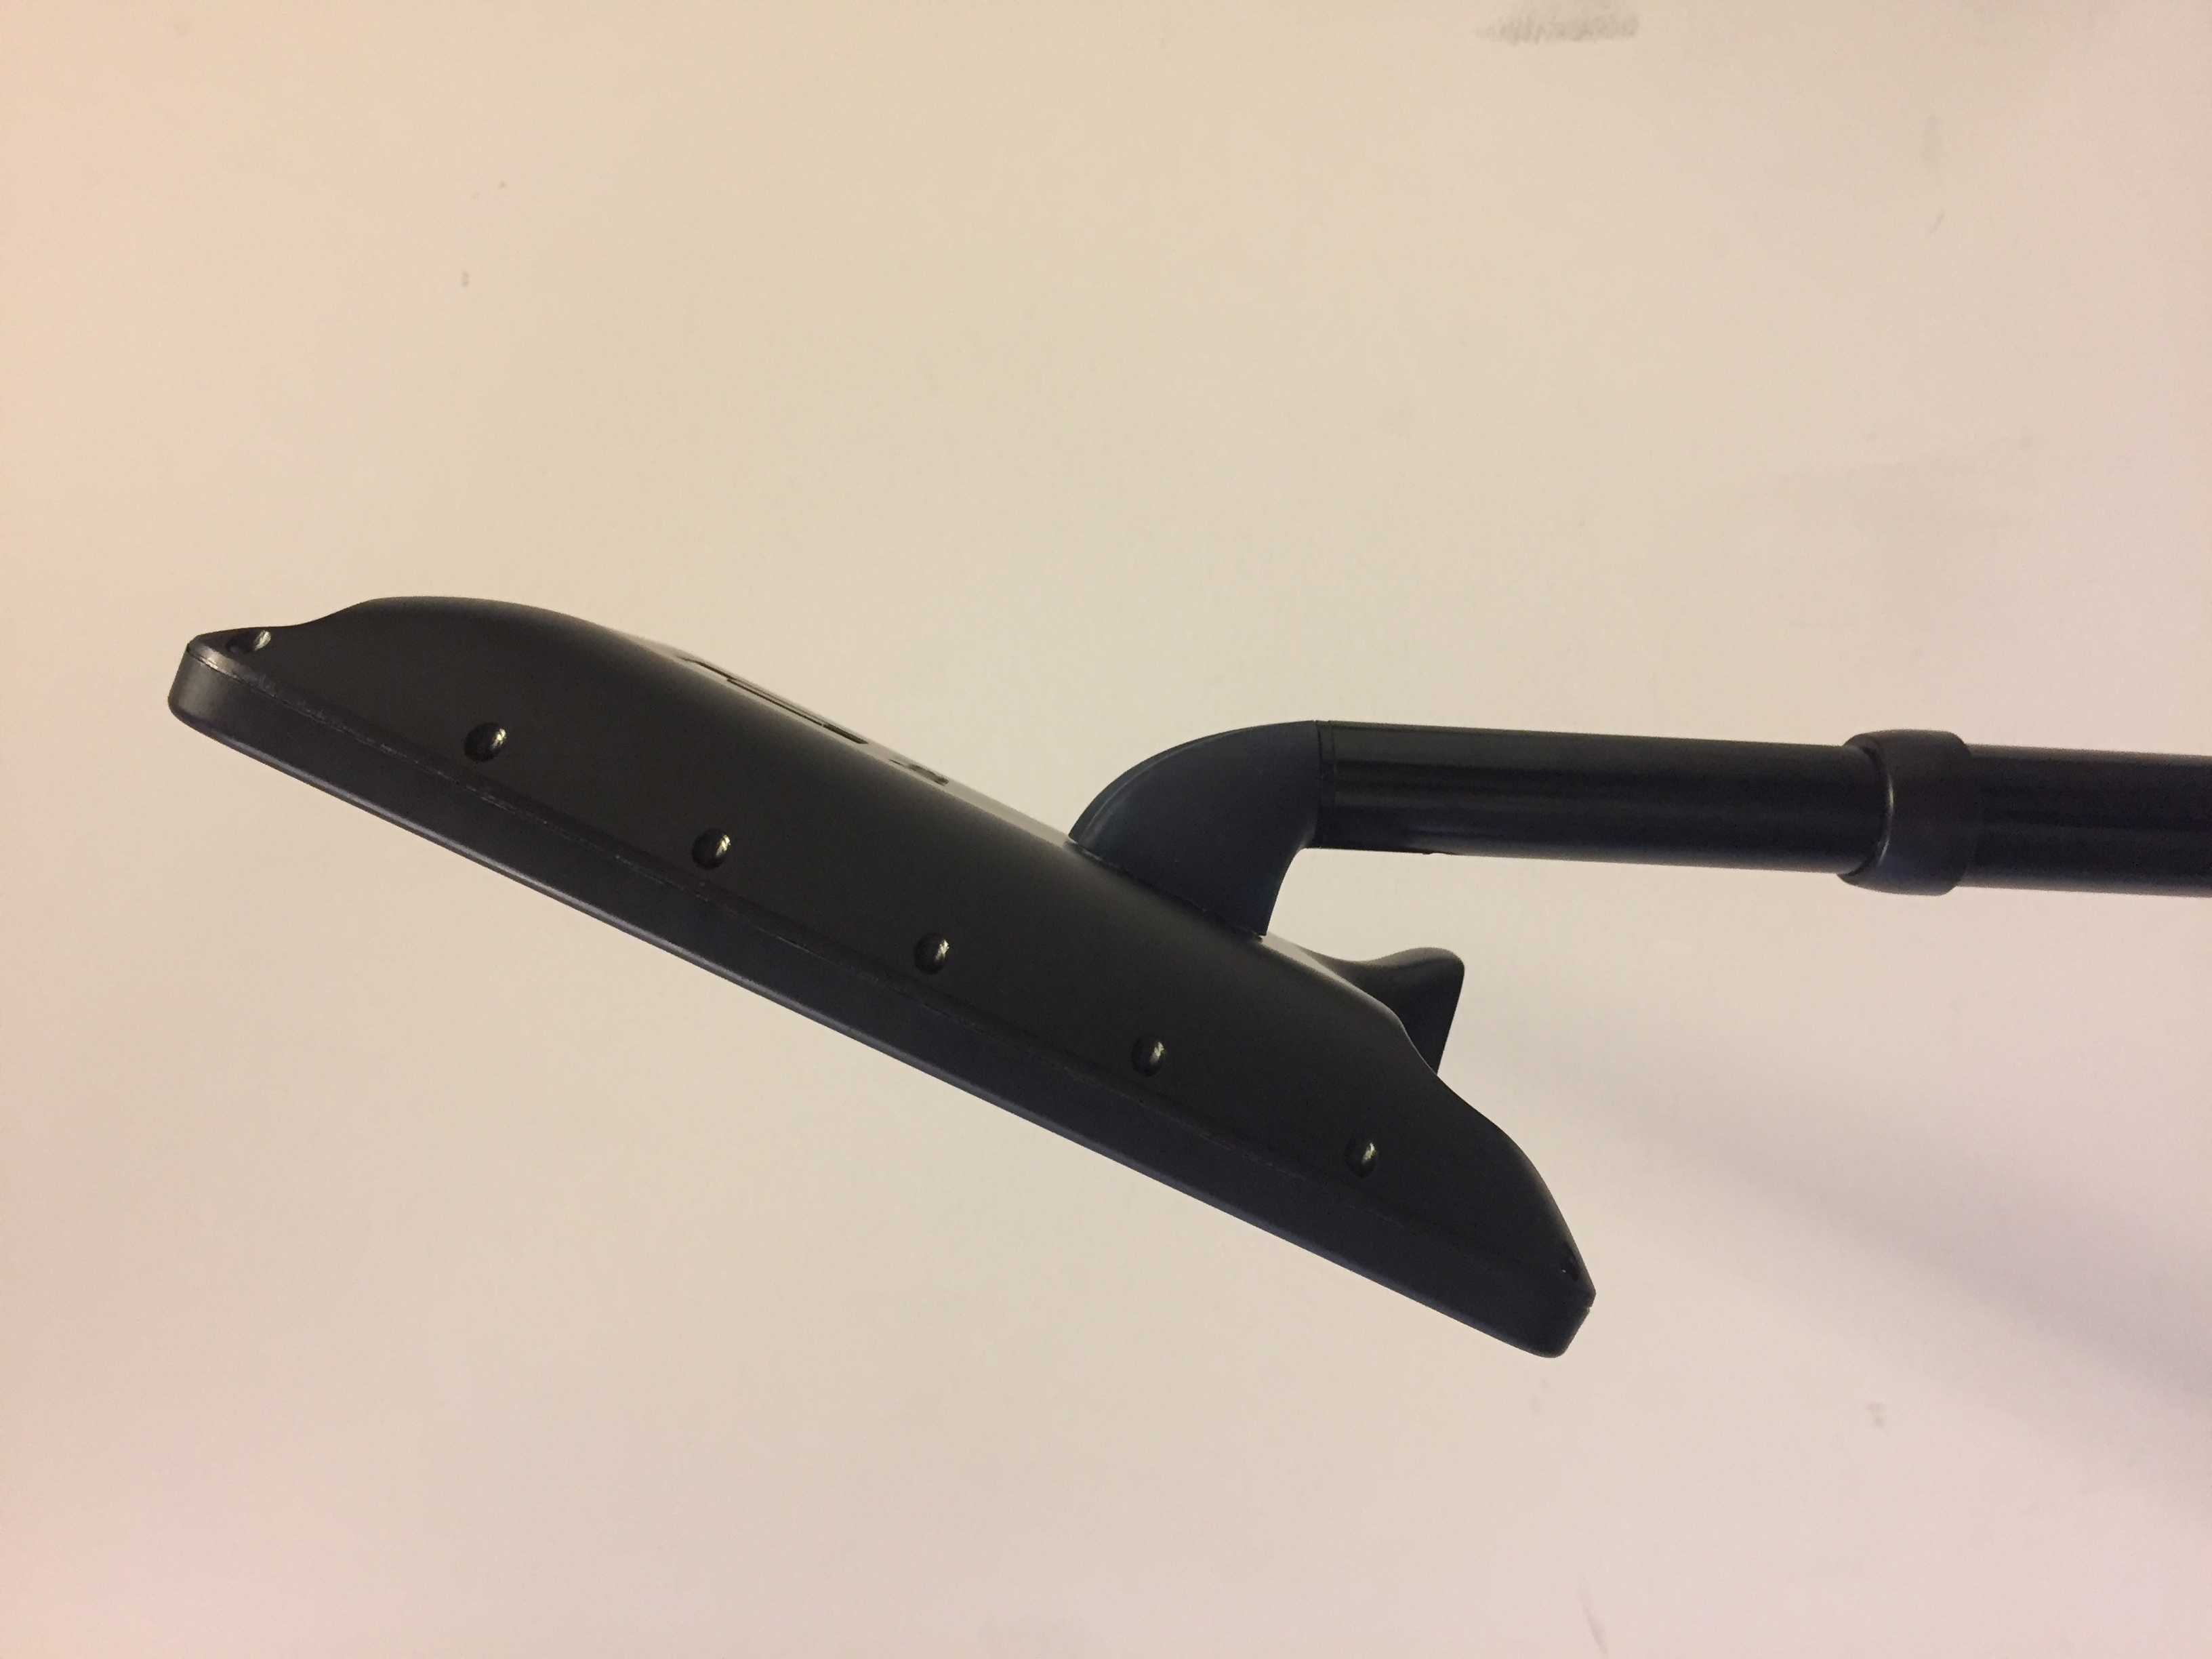
\includegraphics[width=\linewidth, angle =-90]{Figure/ModificeretDoubleSideClose}
  \caption{\textit{Double} profile.}
  \label{fig:ModificeretDoubleSideClose}
\end{minipage}
\end{figure}
\noindent
%
\subsection{Subject Recruitment}
In total the study includes 30 participants from the age of 8 to 62 years (M=37.9, SD=17.1) distributed among 16 females and 14 males. The subjects are recruited by the robot itself, which is remotely controlled by a present observer. The robot approaches potential subjects in the area after the security check. The wireframe on the iPad asks the subjects if it may help them find their way around AAL and presents a "Yes" or "No" option. If "No" is pressed, the robot wishes the traveller a pleasent journey. If "Yes" is pressed, the subjects are presented with four wayfinding options: Food, Shopping, Toilets, or Gate information. The subjects are then asked to kindly follow the robot after they have chosen their preferred option. The robot then leads the subjects to an interviewer who shortly informs them of the study and receives verbal consent to record audio during a semi-structured interview. In total we conducted 18 interviews by which 11 where on a single traveller whereas the remaining seven was on a group of travellers. 
 
\subsection{Semi-structured Interview}
The interview was semi-structured in two parts. The first part consisted of probing the subjects for their first impression and experience of interacting with the robot. The following are only guidance to the conversation topics and not specific questions:\\ 
%
\begin{itemize}
\item First impression of the robot from the recruitment -  Førstehåndsindtryk af robotten - fra rekrutteringen
\item How the robot approaches - Måden hvorpå robotten henvender sig
\item What the subjects think about the robot Hvad testpersonen synes om robotten
\item What the subjects might think other travellers think about the ongoing interaction - Hvad testpersonerne tror andre rejsende tænker om interaktionen 
\item Robot relevans - Robottens relevans
\item Robot reliability - Robottens pålidelighed
\item Experiences at an airport without robot help - Normal oplevelse i en lufthavn uden hjælp fra en robot\\
\end{itemize}
\noindent
%
The second part consisted of asking specific questions relating to the robots physical characteristics like height, approach, and speed. These questions because the variables are known to affect the experience of the HRI.\\
%
\begin{itemize}
\item What is your opinion about - Hvad synes du om..
	\begin{itemize}
		\item Robot speed? - Robottens hastighed?
		\item Robot height? - Robottens højde?
		\item Robot distance to you? - Robottens afstand til dig?
		\item Robot movements? - Robottens generelle bevægelse?
		\item Robot appearance? -  Robottens udseende?
		\item Direction of approach? - Den retning robotten henvendte sig til dig fra?\\
	\end{itemize}
\end{itemize}
%
The two parts was conducted in continuation of each other and the questions in the second part were only asked if the subjects had not previously answered them by themselves.
 
\subsection{Roles}
Five researchers were present during the study at AAL. One controlled the \textit{Double 1} robot, one conducted the interview, and the remaining three observed the travelers as they interacted or walked passed the robot. 

\subsection{Data Processing}
The interviews were transcribed and coded along with observations into affinity notes. The purpose being to create an affinity diagram \cite{Wendell2005}, which brings insights and issues into a wall-sized hierarchical diagram based on subjects' statements and behavior. In the end this affinity diagram will be pivotal in elicitating the variables that affect the HRI according to Danes, and thereafter in creating the scales to be used for further work.




%Real travellers were observed interacting with a robot in AAL and interviewed in order to get a sense of peoples' experience and the words they use to describe interacting with a robot in an airport. In total 30 travellers, including 16 women and 14 men, was interviewed during 18 interviews. 11 interviews were performed including a single traveller, where the remaining seven was done on groups of two or more. The participants' ages range from 8 to 62 years (M=37.9, SD=17.1) and have all been travelling more than once.
%
%During the tests a Double robot was used from Double Robotics Inc. Double is basically a segway merged with an iPad and in this study a new head mount was used, so that the iPad was tilted upwards towards the participants, see figure (indsæt billede af double og referencen hertil). Travellers were shown a wireframe on the iPad, intended to help them find a location in the airport of their choosing. In order to create a natural experience, the robot was used to recruit participants by asking them if it could help them find their way around AAL. When travellers were willing to participate the robot led them to the interviewer instead of the chosen gate or restaurant. By doing this, the interviewer could start the interview by asking participants how their first meeting with the robot was without having to first set the scene for the participants and interfering with the natural first impression.
%
%The user experience is then documented like a contextual field study with observations and a semi-structured interview. The interviews are then transcribed and affinity notes are made for building an affinity diagram. By building an affinity diagram these notes can be sorted into a hierarchy of different categories and subcategories, which will tell the user's perspective of the interaction. The affinity diagram represent some of the main areas that are important for travellers when interacting with the robot. These areas are used to create scales, which then are tested with new users in the airport. After gathering data on the chosen parameters, it can then be evaluated in which degree the different attributes contribute to the overall experience of the interaction and how they relate to each other.
